\documentclass[a4paper,12pt]{article}
\usepackage[left=2.5cm,right=2.5cm,top=2.5cm,bottom=2.5cm]{geometry} % Adjust page margins
\usepackage{xcolor,graphicx,framed}
\usepackage[normalem]{ulem}
\usepackage{amsmath}
\usepackage{gensymb}
\usepackage{array}
%\usepackage{lastpage} % Required to print the total number of pages

\begin{document}

\newcommand{\HRule}{\rule{\linewidth}{0.4mm}} % Defines a new command for the horizontal lines, change thickness here

%----------------------------------------------------------------------------------------
%	HEADING SECTIONS
%----------------------------------------------------------------------------------------

\begin{minipage}{0.7\textwidth}
\begin{flushleft} 
\textsc{Universidad del Valle de Guatemala \\
Campus Central \\
Facultad de Ciencias y Humanidades \\
Departamento de Qu\'imica \\
Segundo ciclo, 2014 \\
Fisicoqu\'imica 1 \\
Profesor: Jonathan van der Henst Solis \\
Correo: jjvan@uvg.edu.gt
}
\end{flushleft}
\end{minipage}
~
\begin{minipage}{0.2\textwidth}
\begin{flushright}

\includegraphics[scale=0.4]{Logo_UVG} % Include a department/university logo
\end{flushright}
\end{minipage}\\

%----------------------------------------------------------------------------------------
%	TITLE SECTION
%----------------------------------------------------------------------------------------

\begin{center}
\HRule \\[0.4cm]
{ \bfseries Soluciones propuestas del examen de diagn\'ostico}\\ % Title of your document
\HRule \\[0.4cm]
\end{center}

%----------------------------------------------------------------------------------------

\begin{enumerate}

 \item Graficar las siguientes funciones, escogiendo un sistema coordenado adecuado:
 \begin{enumerate}
  \item $y=5x-5$ 
\begin{center}
 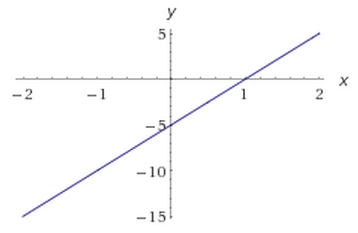
\includegraphics[scale=0.4]{figure1}
\end{center}

  \item $r=\cos\theta$
\begin{center}
 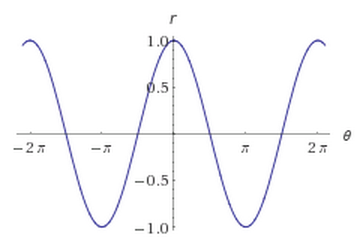
\includegraphics[scale=0.4]{figure2}
\end{center}

  \item $T=\frac{1}{2}mv^2\;(\mbox{considerando a }m\mbox{ como una constante positiva})$
\begin{center}
 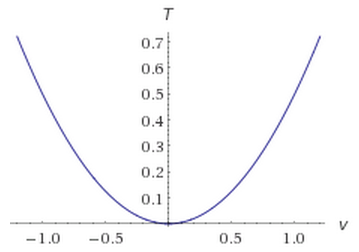
\includegraphics[scale=0.4]{figure3}
\end{center}
Donde el eje vertical est\'a dado en unidades de $m$.

 \end{enumerate}

 \item Derivar la funci\'on $y=x^3e^{2x}$.
$$\frac{dy}{dx}=3x^2e^{2x}+2x^3e^{2x}=(3x^2+2x^3)e^{2x}$$

 \item Usando la ecuaci\'on $PV=nRT$, derivar parcialmente $P$ con respecto a $V$. \\

De primero, expresemos $P$ en funci\'on de $V$:
$$PV=nRT\rightarrow P=\frac{nRT}{V}$$
Derivando parcialmente:
$$\frac{\partial P}{\partial V}=-\frac{nRT}{V^2}$$

 \item Determinar la pendiente de $y=x^2-x$ en $x=3$. \\

Para determinar la pendiente en un punto, se puede determinar la derivada de la funci\'on y luego evaluarla en ese punto.
$$\frac{dy}{dx}=2x-1$$
Evalu\'andola en $x=3$:
$$\frac{dy}{dx}(x=3)=2(3)-1=5$$

 \item Determinar si $y=4x^2-5x+4$ tiene un valor m\'aximo o m\'inimo y encontrarlo, en caso afirmativo. \\

Para determinar si la funci\'on tiene un valor m\'aximo o m\'inimo, se puede buscar alg\'un valor $x$ que haga la primera derivada igual a $0$, confirmando si es m\'aximo o m\'inimo al evaluarlo en la segunda derivada. As\'i que de primero encontremos la primera y la segunda derivada:
$$\frac{dy}{dx}=8x-5$$
$$\frac{d^2y}{dx^2}=\frac{d}{dx}(8x-5)=8$$
Igualando la primera derivada igual a $0$ y despejando:
$$8x-5=0\rightarrow x=\frac{5}{8}$$
Evaluando en la funci\'on, se tiene $y=4\left(\frac{5}{8}\right)^2-5\left(\frac{5}{8}\right)+4=\frac{39}{16}$. Como la segunda derivada es positiva para cualquier valor en $x$, la funci\'on $y$ tiene un m\'inimo en el punto $\left(\frac{5}{8},\frac{39}{16}\right)$, lo cual se puede confirmar al graficarla:

\begin{center}
 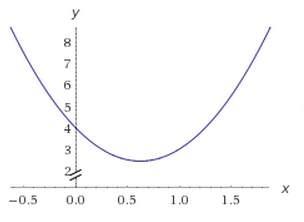
\includegraphics[scale=0.6]{figure4}
\end{center}

 \item Evaluar la integral indefinida $\int \frac{RT}{p} dp$.
$$\int \frac{RT}{p} dp=\frac{1}{RT}\ln |p|+C=\frac{1}{RT}\ln p+C$$
No es necesario incluir el valor absoluto, dado que las presiones no se trabajan con valor negativo.

 \item Evaluar la integral definida $\int_{T_1}^{T_2}\left(a+bT+cT^2+\frac{d}{T}\right)dT$ con $a$, $b$, $c$ y $d$ constantes. 

\begin{tabular}{r c l}
$\int_{T_1}^{T_2}\left(a+bT+cT^2+\frac{d}{T}\right)dT$ & $=$ & $\left.\left(aT+\frac{bT^2}{2}+\frac{cT^3}{3}+d\ln |T|\right)\right|_{T_1}^{T_2}$ \\
& $=$ & $a(T_2-T_1)+\frac{b}{2}(T_2^2-T_1^2)+\frac{c}{3}(T_2^3-T_1^3)+d\ln \left|\frac{T_2}{T_1}\right|$
\end{tabular}

 \item Evaluar $\int_{0}^{2\pi}d\phi$.
$$\int_{0}^{2\pi}d\phi=\left.\phi\right|_{0}^{2\pi}=2\pi-0=2\pi$$

 \item Determinar el error de la masa molar determinada de la siguiente manera:
$$M=\frac{mRT}{PV}=\frac{(1.0339\pm 0.0007\;\text{g})(0.082057\;\text{L}\cdot\text{atm}\cdot\text{mol}^{-1}\cdot\text{K}^{-1})(274.0\pm 0.5\;\text{K})}{(1.036\pm 0.001\;\text{atm})(0.1993\pm 0.0001\;\text{L})}$$ \\

Como las operaciones que se realizan son multiplicaciones y divisiones, la propagaci\'on de error se puede calcular de la siguiente manera:
$$\left(\frac{\Delta M}{M}\right)^2=\left(\frac{\Delta m}{m}\right)^2+\left(\frac{\Delta T}{T}\right)^2+\left(\frac{\Delta P}{P}\right)^2+\left(\frac{\Delta V}{V}\right)^2$$
Sustituyendo con los valores dados:
$$\Delta M=(112.58\;\mbox{g}\cdot\mbox{mol}^{-1})\cdot\sqrt{\left(\frac{0.0007}{1.0339}\right)^2+\left(\frac{0.5}{274.0}\right)^2+\left(\frac{0.001}{1.036}\right)^2+\left(\frac{0.0001}{0.1993}\right)^2}$$
$$\Delta M=(112.58\;\mbox{g}\cdot\mbox{mol}^{-1})\cdot\sqrt{4.58\times10^{-7}+3.33\times10^{-6}+9.32\times10^{-7}+2.52\times 10^{-7}}$$
Con lo que se obtiene un error de la masa molar de $\Delta M=0.25$.

 \item Un recipiente de $1.00$ L se llena con una mezcla de vol\'umenes iguales de ox\'igeno y di\'oxido de nitr\'ogeno a $27\celsius$ y $673$ mm Hg de presi\'on parcial. Se calienta a $420\celsius$ y una vez alcanzado el equilibrio, se encuentran $0.0404$ moles de ox\'igeno. Calcular la constante de equilibrio para el proceso
$$2NO\mbox{(g)}+O_2\mbox{(g)}\rightarrow 2NO_2{(g)}$$
y la presi\'on total de la mezcla. Asumir comportamiento de gas ideal y recordar que $760\;\mbox{mm Hg}=1\;\mbox{atm}$ y que $R=0.082057\;\text{L}\cdot\text{atm}\cdot\text{mol}^{-1}\cdot\text{K}^{-1}$. \\

Asumiendo comportamiento de gases ideales, para determinar las cantidades de gas inicial, dados $P=673\;\mbox{mm Hg}\left(\frac{1\;\mbox{atm}}{760\;\mbox{mm Hg}}\right)=0.8855\;\mbox{atm}$, $V=1.00\;\mbox{L}$ y $T=27\celsius+273.15=300.15\;\mbox{K}$, hacemos:
$$PV=nRT\rightarrow n=\frac{PV}{RT}=\frac{(0.8855\;\mbox{atm})(1.00\;\mbox{L})}{(0.082057\;\text{L}\cdot\text{atm}\cdot\text{mol}^{-1}\cdot\text{K}^{-1})(300.15\;\mbox{K})}=0.0360\;\mbox{mol}$$
que es el n\'umero de moles iniciales tanto del ox\'igeno como del di\'oxido de nitr\'ogeno.

El equilibrio vendr\'a dado por:

\begin{center}
\begin{tabular}{c c c c c c}
& $2NO(g)$ & $+$ & $O_2(g)$ & $\rightarrow$ & $2NO_2(g)$ \\
$n_{iniciales}$ & 0 & & 0.0360 & & 0.0360 \\
$n_{cambio}$ & $2x$ & & $x$ & & $-2x$ \\
$n_{equilibrio}$ & $2x$ & & $0.0404$ & & $0.0360-2x$
\end{tabular}
\end{center}

Con las cantidades de ox\'igeno encontramos que: 
$$n_{O_2}=0.0360+x=0.0404\rightarrow x=4.4\times 10^{-3}$$
La cantidad de moles finales de cada uno ser\'ia: $n_{NO}=2(4.4\times 10^{-3})=8.8\times 10^{-3}\;\mbox{mol}$, $n_{O_2}=0.0404$ y $n_{NO_2}=0.0360-2(4.4\times 10^{-3})=0.0272\;\mbox{mol}$. La cantidad total de moles ser\'ia: $n_T=n_{NO}+n_{O_2}+n_{NO_2}=8.8\times 10^{-3}+0.0404+0.0272=0.0764\;\mbox{mol}$, con lo cual la presi\'on total ser\'ia (usando $T=420\celsius+273.15=693.15\;\mbox{K}$):
$$P_T=\frac{n_TRT}{V}=\frac{(0.0764\;\mbox{mol})(0.082057\;\text{L}\cdot\text{atm}\cdot\text{mol}^{-1}\cdot\text{K}^{-1})(693.15\;\mbox{K})}{1.00\;\mbox{L}}=4.35\;\mbox{atm}$$

Usando fracciones molares, se puede calcular la constante de equilibrio, $K_P$, de la siguiente manera:

$$K_P=\frac{P_{NO_2}^2}{P_{NO}^2\cdot P_{O_2}}=\frac{x_{NO_2}^2P_T^2}{x_{NO}^2P_T^2\cdot x_{O_2}P_T}$$
$$K_P = \frac{\left(\frac{0.0272}{0.0764}\right)^2}{\left(\frac{8.8\times 10^{-3}}{0.0764}\right)^2\cdot\left(\frac{0.0404}{0.0764}\right)(4.35\;\mbox{atm})}=4.15$$

\end{enumerate}
 
\end{document}
